% 第2章 状态空间与搜索基础
\chapter{状态空间与搜索基础}
\label{chap:search}

状态空间搜索是任务规划的理论基础。本章将介绍状态空间的形式化表示方法,以及各种搜索算法。

\section{状态空间表示}

\subsection{状态的形式化定义}

\begin{definition}[状态]
    状态(State)是对系统在某一时刻所处情况的完整描述。在规划问题中,状态通常用一组\keyterm{状态变量}(State Variables)或\keyterm{命题}(Propositions)来表示。
\end{definition}

以积木世界为例,假设有三个积木A、B、C和一个桌面Table。我们可以用以下谓词来描述状态:
\begin{itemize}
    \item $\text{On}(x, y)$:积木$x$在$y$上面
    \item $\text{OnTable}(x)$:积木$x$在桌面上
    \item $\text{Clear}(x)$:积木$x$上面没有其他积木
    \item $\text{Holding}(x)$:机械手正在抓取积木$x$
    \item $\text{ArmEmpty}$:机械手是空的
\end{itemize}

一个具体的状态可以表示为这些谓词的集合:
\begin{equation}
    s_0 = \{\text{OnTable}(A), \text{On}(B, A), \text{Clear}(B), \text{OnTable}(C), \text{Clear}(C), \text{ArmEmpty}\}
\end{equation}

\subsection{动作与状态转移}

\begin{definition}[动作]
    动作(Action)是智能体可以执行的操作,它将系统从一个状态转移到另一个状态。一个动作$a$可以用三元组$\langle \text{Pre}(a), \text{Add}(a), \text{Del}(a) \rangle$来描述:
    \begin{itemize}
        \item $\text{Pre}(a)$:前提条件,动作执行前必须满足的条件
        \item $\text{Add}(a)$:添加列表,动作执行后新增的事实
        \item $\text{Del}(a)$:删除列表,动作执行后删除的事实
    \end{itemize}
\end{definition}

\begin{example}[积木世界的动作定义]
    \textbf{拾取动作} $\text{PickUp}(x)$:从桌面上拾取积木$x$
    \begin{align}
        \text{Pre} &: \{\text{OnTable}(x), \text{Clear}(x), \text{ArmEmpty}\} \\
        \text{Add} &: \{\text{Holding}(x)\} \\
        \text{Del} &: \{\text{OnTable}(x), \text{ArmEmpty}\}
    \end{align}

    \textbf{放下动作} $\text{PutDown}(x)$:将手中的积木$x$放到桌面上
    \begin{align}
        \text{Pre} &: \{\text{Holding}(x)\} \\
        \text{Add} &: \{\text{OnTable}(x), \text{Clear}(x), \text{ArmEmpty}\} \\
        \text{Del} &: \{\text{Holding}(x)\}
    \end{align}

    \textbf{堆叠动作} $\text{Stack}(x, y)$:将手中的积木$x$放到积木$y$上
    \begin{align}
        \text{Pre} &: \{\text{Holding}(x), \text{Clear}(y)\} \\
        \text{Add} &: \{\text{On}(x, y), \text{Clear}(x), \text{ArmEmpty}\} \\
        \text{Del} &: \{\text{Holding}(x), \text{Clear}(y)\}
    \end{align}

    \textbf{拆卸动作} $\text{Unstack}(x, y)$:从积木$y$上取下积木$x$
    \begin{align}
        \text{Pre} &: \{\text{On}(x, y), \text{Clear}(x), \text{ArmEmpty}\} \\
        \text{Add} &: \{\text{Holding}(x), \text{Clear}(y)\} \\
        \text{Del} &: \{\text{On}(x, y), \text{ArmEmpty}\}
    \end{align}
\end{example}

\begin{definition}[状态转移函数]
    给定状态$s$和动作$a$,如果$\text{Pre}(a) \subseteq s$,则$a$在$s$中是\keyterm{可应用的}(Applicable)。状态转移函数$\gamma$定义为:
    \begin{equation}
        \gamma(s, a) = (s \setminus \text{Del}(a)) \cup \text{Add}(a)
    \end{equation}
\end{definition}

\subsection{目标状态与规划问题}

\begin{definition}[规划问题]
    一个\keyterm{经典规划问题}可以定义为三元组 $\mathcal{P} = \langle \mathcal{D}, s_0, g \rangle$,其中:
    \begin{itemize}
        \item $\mathcal{D}$是规划领域,包括状态变量和动作定义
        \item $s_0$是初始状态
        \item $g$是目标条件(一组必须满足的命题)
    \end{itemize}
\end{definition}

\begin{definition}[解(规划)]
    规划问题$\mathcal{P}$的解是一个动作序列$\pi = \langle a_1, a_2, \ldots, a_n \rangle$,使得:
    \begin{enumerate}
        \item $a_1$在$s_0$中可应用
        \item 对于$i = 1, \ldots, n-1$,$a_{i+1}$在$\gamma(\cdots\gamma(\gamma(s_0, a_1), a_2)\cdots, a_i)$中可应用
        \item $g \subseteq \gamma(\cdots\gamma(\gamma(s_0, a_1), a_2)\cdots, a_n)$
    \end{enumerate}
\end{definition}

\section{盲目搜索策略}

\keyterm{盲目搜索}(Uninformed Search)也称为无信息搜索,是指在搜索过程中不使用问题特定知识的搜索方法。

\subsection{广度优先搜索}

\keyterm{广度优先搜索}(Breadth-First Search,BFS)按层次顺序扩展节点,先扩展所有深度为$d$的节点,再扩展深度为$d+1$的节点。

\begin{algorithm}[H]
    \caption{广度优先搜索}
    \label{alg:bfs}
    \KwIn{规划问题 $\mathcal{P} = \langle \mathcal{D}, s_0, g \rangle$}
    \KwOut{解(动作序列)或失败}

    $\text{frontier} \gets$ 队列,初始包含 $(s_0, \langle\rangle)$\;
    $\text{explored} \gets \emptyset$\;

    \While{$\text{frontier}$ 非空}{
        $(s, \pi) \gets \text{frontier.dequeue}()$\;
        \If{$g \subseteq s$}{
            \KwRet{$\pi$}
        }
        $\text{explored} \gets \text{explored} \cup \{s\}$\;
        \ForEach{动作 $a$ 在 $s$ 中可应用}{
            $s' \gets \gamma(s, a)$\;
            \If{$s' \notin \text{explored}$ 且 $s' \notin \text{frontier}$}{
                $\text{frontier.enqueue}((s', \pi \cdot \langle a \rangle))$\;
            }
        }
    }
    \KwRet{失败}
\end{algorithm}

\textbf{性质分析}:
\begin{itemize}
    \item \textbf{完备性}:如果解存在,BFS一定能找到
    \item \textbf{最优性}:BFS找到的解是步数最少的(假设所有动作代价相同)
    \item \textbf{时间复杂度}:$O(b^d)$,其中$b$是分支因子,$d$是解的深度
    \item \textbf{空间复杂度}:$O(b^d)$
\end{itemize}

\subsection{深度优先搜索}

\keyterm{深度优先搜索}(Depth-First Search,DFS)总是扩展搜索树中最深的节点。

\begin{algorithm}[H]
    \caption{深度优先搜索}
    \label{alg:dfs}
    \KwIn{规划问题 $\mathcal{P} = \langle \mathcal{D}, s_0, g \rangle$}
    \KwOut{解(动作序列)或失败}

    $\text{frontier} \gets$ 栈,初始包含 $(s_0, \langle\rangle)$\;
    $\text{explored} \gets \emptyset$\;

    \While{$\text{frontier}$ 非空}{
        $(s, \pi) \gets \text{frontier.pop}()$\;
        \If{$g \subseteq s$}{
            \KwRet{$\pi$}
        }
        $\text{explored} \gets \text{explored} \cup \{s\}$\;
        \ForEach{动作 $a$ 在 $s$ 中可应用}{
            $s' \gets \gamma(s, a)$\;
            \If{$s' \notin \text{explored}$}{
                $\text{frontier.push}((s', \pi \cdot \langle a \rangle))$\;
            }
        }
    }
    \KwRet{失败}
\end{algorithm}

\textbf{性质分析}:
\begin{itemize}
    \item \textbf{完备性}:在有限状态空间中完备(需要避免重复状态)
    \item \textbf{最优性}:不保证最优
    \item \textbf{时间复杂度}:$O(b^m)$,其中$m$是状态空间的最大深度
    \item \textbf{空间复杂度}:$O(bm)$
\end{itemize}

\subsection{迭代加深搜索}

\keyterm{迭代加深搜索}(Iterative Deepening Search,IDS)结合了BFS的完备性和DFS的空间效率。

\begin{algorithm}[H]
    \caption{迭代加深搜索}
    \label{alg:ids}
    \KwIn{规划问题 $\mathcal{P}$}
    \KwOut{解或失败}

    \For{$\text{depth} \gets 0$ \KwTo $\infty$}{
        $\text{result} \gets \text{DepthLimitedSearch}(\mathcal{P}, \text{depth})$\;
        \If{$\text{result} \neq \text{cutoff}$}{
            \KwRet{$\text{result}$}
        }
    }
\end{algorithm}

\begin{example}[八数码问题求解]
\label{ex:8puzzle}
    八数码问题(8-Puzzle)是一个经典的搜索问题。在$3 \times 3$的棋盘上有8个编号为1--8的滑块和一个空格,目标是通过移动滑块将棋盘从初始状态变换到目标状态。

    初始状态:
    \begin{center}
    \begin{tabular}{|c|c|c|}
        \hline
        2 & 8 & 3 \\
        \hline
        1 & 6 & 4 \\
        \hline
        7 &   & 5 \\
        \hline
    \end{tabular}
    \end{center}

    目标状态:
    \begin{center}
    \begin{tabular}{|c|c|c|}
        \hline
        1 & 2 & 3 \\
        \hline
        8 &   & 4 \\
        \hline
        7 & 6 & 5 \\
        \hline
    \end{tabular}
    \end{center}

    \textbf{状态表示}:用9元组$(p_1, p_2, \ldots, p_9)$表示,其中$p_i$是位置$i$上的滑块编号(0表示空格)。

    \textbf{动作}:上、下、左、右(移动空格)。

    \textbf{搜索结果比较}:
    \begin{center}
    \begin{tabular}{lrr}
        \toprule
        算法 & 扩展节点数 & 解的长度 \\
        \midrule
        BFS & 约46,000 & 23 \\
        DFS & 可能很大 & 不确定 \\
        IDS & 约47,000 & 23 \\
        \bottomrule
    \end{tabular}
    \end{center}
\end{example}

\section{启发式搜索}

\keyterm{启发式搜索}(Heuristic Search)利用问题特定的知识来引导搜索方向,从而提高搜索效率。

\subsection{启发函数设计}

\begin{definition}[启发函数]
    启发函数$h: S \to \mathbb{R}_{\geq 0}$估计从状态$s$到达目标状态的代价。如果$h(s) = 0$当且仅当$s$满足目标条件,则$h$是\keyterm{目标感知的}(Goal-Aware)。
\end{definition}

\begin{definition}[可采纳启发式]
    如果对于所有状态$s$,$h(s) \leq h^*(s)$,其中$h^*(s)$是从$s$到目标的真实最优代价,则$h$是\keyterm{可采纳的}(Admissible)。
\end{definition}

\begin{definition}[一致启发式]
    如果对于所有状态$s$和动作$a$,$h(s) \leq c(s, a) + h(\gamma(s, a))$,其中$c(s, a)$是执行$a$的代价,则$h$是\keyterm{一致的}(Consistent)。
\end{definition}

\subsection{A*算法}

\keyterm{A*算法}是最著名的启发式搜索算法,它使用评估函数$f(s) = g(s) + h(s)$来选择下一个扩展的节点,其中$g(s)$是从初始状态到$s$的实际代价。

\begin{algorithm}[H]
    \caption{A*算法}
    \label{alg:astar}
    \KwIn{规划问题 $\mathcal{P}$,启发函数 $h$}
    \KwOut{最优解或失败}

    $\text{open} \gets$ 优先队列,按$f$值排序,初始包含 $(s_0, \langle\rangle, 0)$\;
    $\text{closed} \gets \emptyset$\;

    \While{$\text{open}$ 非空}{
        $(s, \pi, g) \gets \text{open.extractMin}()$\;
        \If{$g \subseteq s$}{
            \KwRet{$\pi$}
        }
        \If{$s \in \text{closed}$}{
            \textbf{continue}\;
        }
        $\text{closed} \gets \text{closed} \cup \{s\}$\;
        \ForEach{动作 $a$ 在 $s$ 中可应用}{
            $s' \gets \gamma(s, a)$\;
            $g' \gets g + c(s, a)$\;
            \If{$s' \notin \text{closed}$}{
                $\text{open.insert}((s', \pi \cdot \langle a \rangle, g'))$\;
            }
        }
    }
    \KwRet{失败}
\end{algorithm}

\begin{theorem}
    如果启发函数$h$是可采纳的,则A*算法返回的解是最优的。
\end{theorem}

\begin{theorem}
    如果启发函数$h$是一致的,则A*算法在扩展每个节点时,已经找到了到达该节点的最优路径。
\end{theorem}

\subsection{IDA*算法}

\keyterm{IDA*}(Iterative Deepening A*)是A*的迭代加深版本,用深度限制代替优先队列,节省了空间。

\begin{example}[路径规划中的A*应用]
\label{ex:pathfinding}
    考虑在一个$10 \times 10$的网格地图中,从起点$(1,1)$到达终点$(10,10)$,地图中有障碍物。

    \textbf{状态}:机器人当前位置$(x, y)$

    \textbf{动作}:上、下、左、右移动(代价为1)或对角线移动(代价为$\sqrt{2}$)

    \textbf{启发函数}:常用的启发函数包括:
    \begin{itemize}
        \item \textbf{曼哈顿距离}:$h_1(s) = |x - x_g| + |y - y_g|$(仅考虑四方向移动时可采纳)
        \item \textbf{欧几里得距离}:$h_2(s) = \sqrt{(x - x_g)^2 + (y - y_g)^2}$(总是可采纳)
        \item \textbf{切比雪夫距离}:$h_3(s) = \max(|x - x_g|, |y - y_g|)$(考虑对角移动时可采纳)
    \end{itemize}

    图\ref{fig:astar-example}展示了使用不同启发函数时A*算法的搜索过程。
\end{example}

\begin{figure}[htbp]
    \centering
    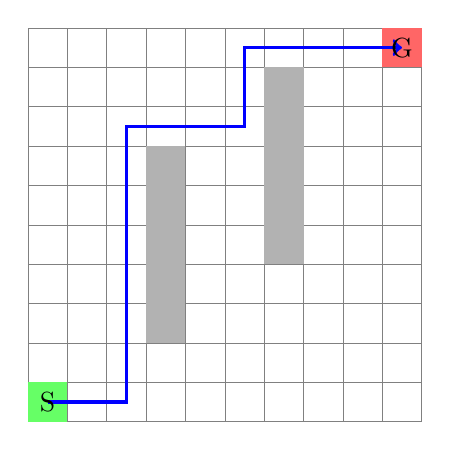
\begin{tikzpicture}[scale=0.5]
        % 网格
        \draw[step=1,gray,very thin] (0,0) grid (10,10);

        % 障碍物
        \fill[black!30] (3,2) rectangle (4,7);
        \fill[black!30] (6,4) rectangle (7,9);

        % 起点和终点
        \fill[green!60] (0,0) rectangle (1,1);
        \fill[red!60] (9,9) rectangle (10,10);

        % 路径
        \draw[blue,very thick,->] (0.5,0.5) -- (2.5,0.5) -- (2.5,1.5) -- (2.5,7.5) -- (5.5,7.5) -- (5.5,9.5) -- (9.5,9.5);

        % 标签
        \node at (0.5,0.5) {S};
        \node at (9.5,9.5) {G};
    \end{tikzpicture}
    \caption{网格地图中的A*路径规划示例}
    \label{fig:astar-example}
\end{figure}

\section{搜索算法的性能分析}

\subsection{完备性与最优性}

\begin{table}[htbp]
    \centering
    \caption{搜索算法性能比较}
    \label{tab:search-comparison}
    \begin{tabular}{lcccc}
        \toprule
        算法 & 完备性 & 最优性 & 时间复杂度 & 空间复杂度 \\
        \midrule
        BFS & 是 & 是$^*$ & $O(b^d)$ & $O(b^d)$ \\
        DFS & 否$^{**}$ & 否 & $O(b^m)$ & $O(bm)$ \\
        IDS & 是 & 是$^*$ & $O(b^d)$ & $O(bd)$ \\
        A* & 是 & 是$^{***}$ & $O(b^d)$ & $O(b^d)$ \\
        IDA* & 是 & 是$^{***}$ & $O(b^d)$ & $O(bd)$ \\
        \bottomrule
    \end{tabular}

    \footnotesize{$^*$假设所有动作代价相同;$^{**}$在无限空间中不完备;$^{***}$要求启发函数可采纳}
\end{table}

\subsection{时间复杂度与空间复杂度}

规划问题的计算复杂性是一个重要的理论问题。

\begin{theorem}
    经典规划问题(判定版本)是PSPACE完全的。
\end{theorem}

这意味着规划问题在最坏情况下非常困难。然而,实际问题往往具有特殊结构,可以用启发式方法高效求解。

\section*{本章小结}

本章介绍了状态空间搜索的基本概念和算法。状态空间由状态、动作和转移函数组成。盲目搜索算法(BFS、DFS、IDS)不使用问题特定知识,而启发式搜索(A*、IDA*)利用启发函数引导搜索。选择合适的搜索算法和启发函数对规划系统的效率至关重要。

\section*{习题}

\begin{enumerate}
    \item 对于示例\ref{ex:8puzzle}中的八数码问题,设计两种不同的启发函数,并分析其可采纳性。

    \item 证明:如果启发函数$h$是一致的,则$h$必定是可采纳的。

    \item 实现BFS和A*算法,求解15数码问题,比较两者的性能。

    \item 考虑一个机器人在$n \times n$网格中导航的问题,分析以下情况下A*算法的时间复杂度:
    \begin{enumerate}
        \item 使用$h(s) = 0$(退化为Dijkstra算法)
        \item 使用完美启发函数$h(s) = h^*(s)$
    \end{enumerate}

    \item 设计一个规划问题,使得DFS比BFS效率更高,并解释原因。
\end{enumerate}
